\documentclass{article}
\usepackage[margin=1in]{geometry}
\usepackage[utf8]{inputenc}
\usepackage{graphicx}
\usepackage{subfigure}
\usepackage{color}
\usepackage{amssymb, amsmath}
\usepackage{array}
\usepackage[normalem]{ulem}
\usepackage{titling}
\usepackage{url}
\usepackage[colorlinks=true, urlcolor=blue, linkcolor=red]{hyperref}
\usepackage{float}
\usepackage{dialogue}
\usepackage{amsmath}
\usepackage{algorithm}
\usepackage{algpseudocode}


\usepackage{cite}
\newcommand{\subtitle}[1]{%
 \posttitle{%
 \par\end{center}
 \begin{center}\large#1\end{center}
 \vskip0.5em}%
}


\begin{document}

\title{Particle Filter Experiments}
\subtitle{github: \url{https://github.com/helenlu66/ParticleFilter}}
\author{Helen Lu}
\maketitle


\section{Algorithm}
Repeat steps 3-18 for each time step $t$:
\hrulefill

\begin{algorithm}
\caption{Particle Filter}
\begin{algorithmic}[1]
    \State \textbf{Initialization:}
        \State Draw a sample of $N$ particles uniformly distributed in the map's 2D plane.
        \State Assign equal weights: $w_0^{(i)} = \frac{1}{N}$.
    \State \textbf{Move:}
        \For{each particle $i$ from $1$ to $N$}
            \State move by applying the movement vector and add some randomness $(x_t^{(i)}, y_t^{(i)}) = (x_{t-1}^{(i)}, y_{t-1}^{(i)}) + (dx, dy) + (N(0, \sigma^2), N(0, \sigma^2))$ .
        \EndFor
    \State \textbf{Update Weights:}
        \State Observe the reference image at the true location
        \State Get a GPS reading of the true location
        \For{each particle $i$ from $1$ to $N$}
            \State Observe the image at $(x_t^{(i)}, y_t^{(i)})$, calculate similarity to reference image using the Structural Similarity Index (SSIM) $ssim(image^{(i)}, image_{ref})$ 
            \State Calculate closeness (1.0 - normalized Euclidean distance away from GPS reading): $close(state^{(i)} - state_{gps}) = 1.0 - norm_dist(state^{(i)} - state_{gps})$.
            \State Calculate a composite score for similarity: $sim(obs, ref) = (1.0 - \gamma) * ssim(image^{(i)}, image_{ref}) + \gamma * close(state^{(i)} - state_{gps})$ \Comment{$\gamma$ is a hyperparameter we can tune}
        \EndFor
    \State \textbf{Roulette Resample:}
        \State Resample $N * 95\%$ particles from the current set based on their weights to form a new set of particles.
        \State Add $N * 5\%$ random particles to the resampled particles
    \State \textbf{Evaluate:}
        \State Calculate the Mean Squared Error of the top $10\%$ nearest neighbors.
\end{algorithmic}
\label{Particle Filter Algorithm}
\end{algorithm}
\hrulefill


The particle filter algorithm used for the experiments is described in the pseudocode \ref{Particle Filter Algorithm}. We used a composite score for estimating $p(z|x)$. We calculate the composite score by combining the similarity between the particle's image and the reference image with the closeness of the particle's location to the GPS reading of the true location: $sim(obs, ref) = (1.0 - \gamma) * ssim(image^{(i)}, image_{ref}) + \gamma * close(state^{(i)} - state_{gps})$. The similarity between the particle's image and the reference image is measured using the Structurl Similarity Index. We explore different values of $\gamma$ in the experiments section.
\subsection{Extra Credits Attempted}
We incorporated noisy GPS readings (noise drawn from normal distribution centered at 0.0 with variance of 1.0), implemented a weighted distance-based and image observation based similarity measure, and experimented with white noise.
\section{Experiments}
The experiments explore changes in the following conditions:
\begin{itemize}
    \item the observation size: 25, 50, 100
    \item the number of particles: 100, 500, 1000
    \item the weight used to produce the composite similarity score: 0.0, 0.2, 0.5, 0.8, 1.0
    \item the level of white noise added to the reference image: 0.0, 0.05, 0.1, 0.25, 0.5, 0.75, 1.0
\end{itemize}
\begin{figure*}[!ht]
    \centering
    \vspace{-0.3cm}
    \subfigure[Bay Map MSE Curves for Different Observation Image Sizes] {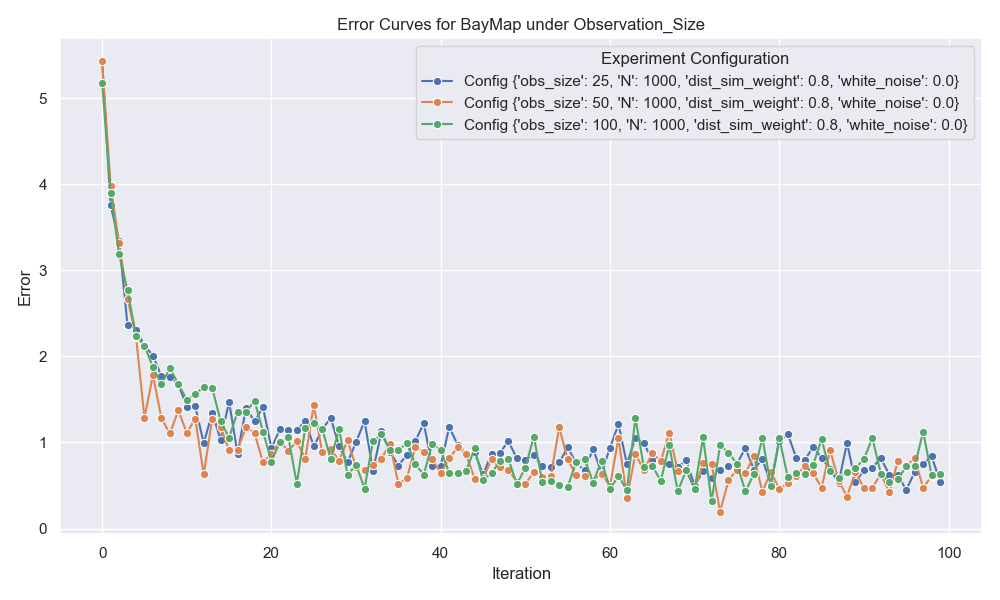
\includegraphics[width=0.49\linewidth]{plots/BayMap_Observation_Size.png}\label{fig:bay_obs_size}}\hspace{0.2cm}%
    \subfigure[Bay Map MSE Curves for Different Particle Number] {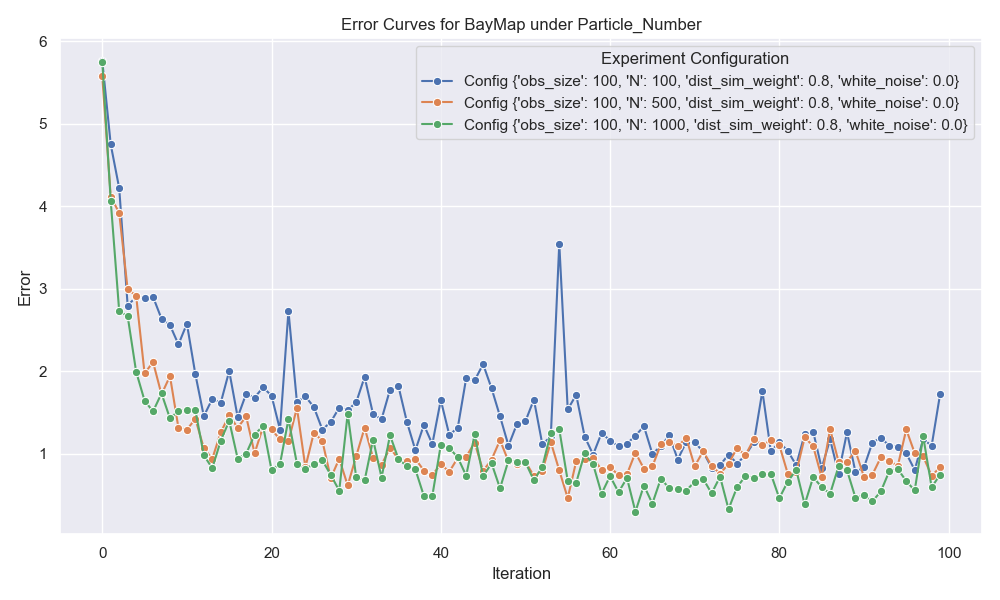
\includegraphics[width=0.49\linewidth]{plots/BayMap_Particle_Number.png}\label{fig:bay_pnum}}\hspace{0.2cm}%
    \subfigure[Bay Map MSE Curves for Different Composite Score Weights] {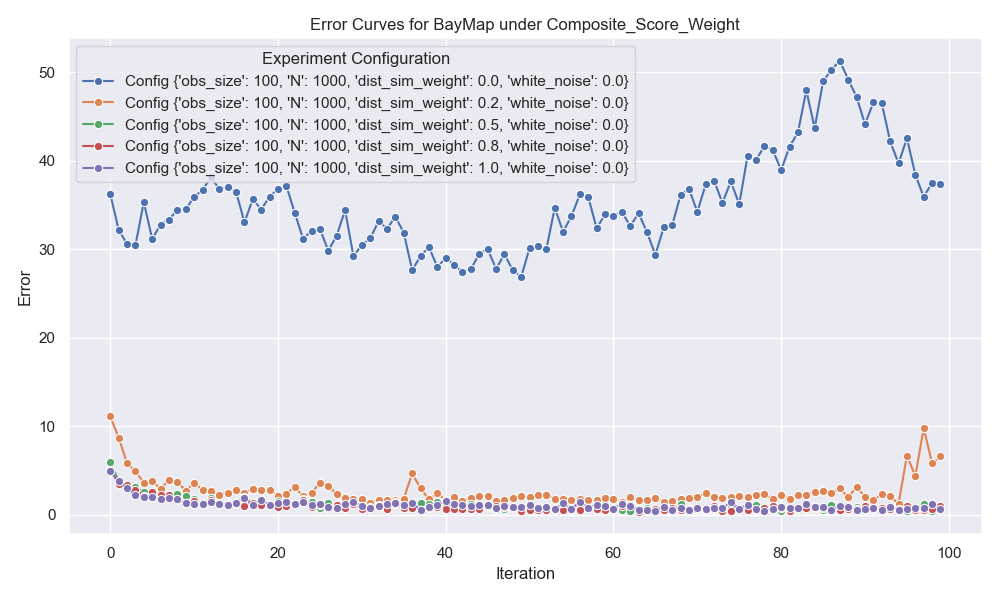
\includegraphics[width=0.49\linewidth]{plots/BayMap_Composite_Score_Weight.png}\label{fig:bay_scoreweight}}\hspace{0.2cm}%
    \subfigure[Bay Map MSE Curves for Different White Noise Levels] {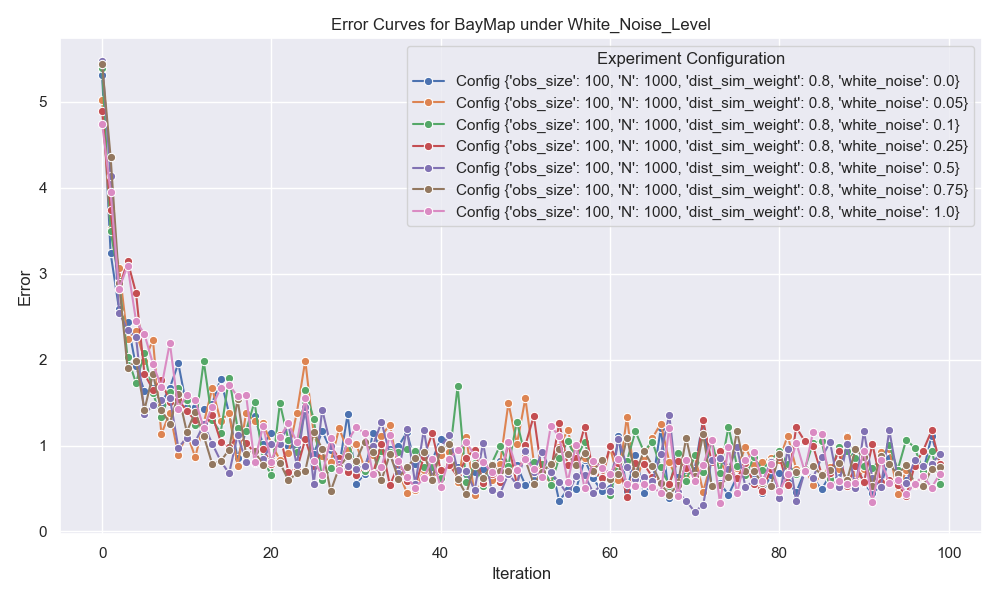
\includegraphics[width=0.49\linewidth]{plots/BayMap_White_Noise_Level.png}\label{fig:bay_noise}}\hspace{0.2cm}%
    \vspace{-0.4cm}
    \caption{MSE Curves for Bay Map}
    \label{fig:bay}
    \vspace{-0.3cm}
\end{figure*}
The default configuration sets the observation image size to 100, the number of particles to 1000, the weight used in the composite score to 0.8, and the white noise level to 0.0. In each experiment condition, we vary the level of one variable. The other variables remain the same levels as that of the default configuration. We run 10 trials per level per condiiton and average across trials to get the error curves. The error is the mean squared error between the true location and the k nearest neighbors with the k being set to 10\% of the number of particles. At each timestep, the filter gets a GPS location with added Gaussian noise centered around 0 with variance=1.0. We also circle the particles and the true locations on the map every 10 iterations to see if the particles are clustering around the true locations. Images generated from the experiments for each map are in the github repository in the directory named after the map.
\section{Results}
\begin{figure}[!ht]
    \centering
    \includegraphics[width=0.55\linewidth]{BayMap/obs_size100/pnum1000/score_weight0.0/noise0.0/step90weights.png}
    \label{fig:bay_scoreweight0_particles_sample_iter90}\caption{Bay Map Particles Clustering to the Wrong Location When $\gamma$=0.0}
\end{figure}
\begin{figure*}[!ht]
    \centering
    \vspace{-0.3cm}
    \subfigure[Mario Map MSE Curves for Different Observation Image Sizes] {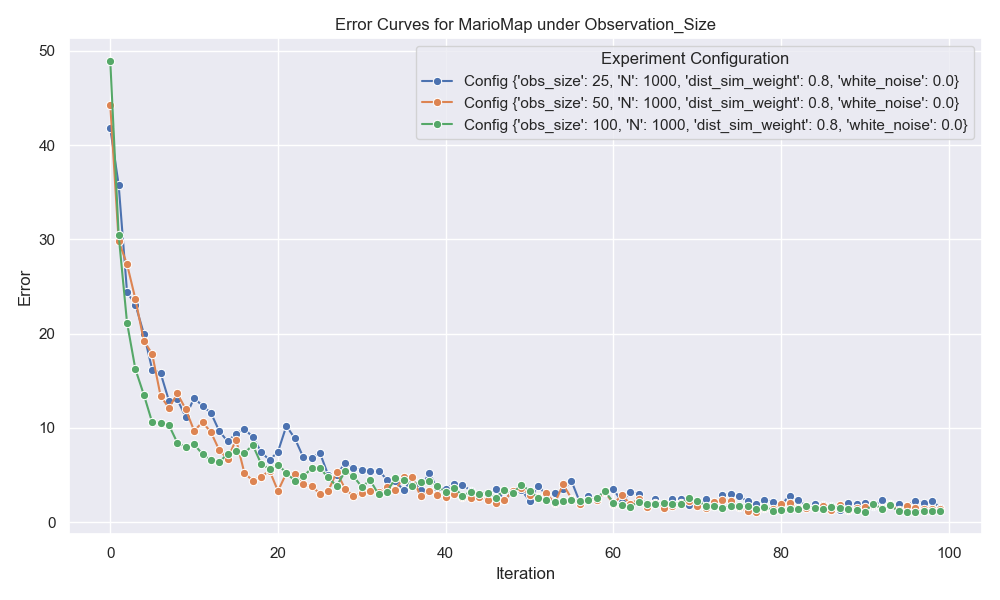
\includegraphics[width=0.49\linewidth]{plots/MarioMap_Observation_Size.png}\label{fig:mario_obs_size}}\hspace{0.2cm}%
    \subfigure[Mario Map MSE Curves for Different Particle Number] {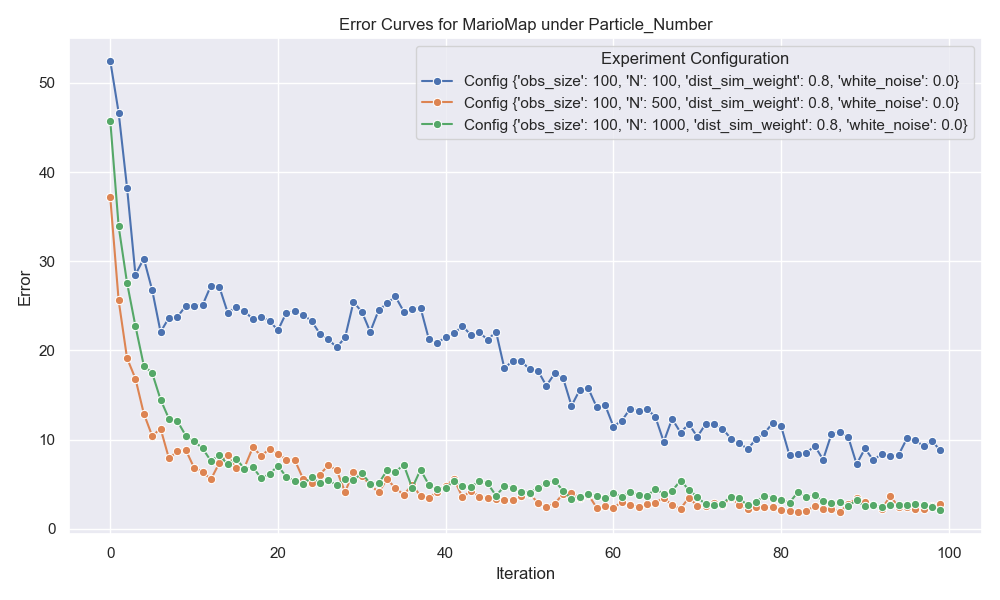
\includegraphics[width=0.49\linewidth]{plots/MarioMap_Particle_Number.png}\label{fig:mario_pnum}}\hspace{0.2cm}%
    \subfigure[Mario Map MSE Curves for Different Composite Score Weights] {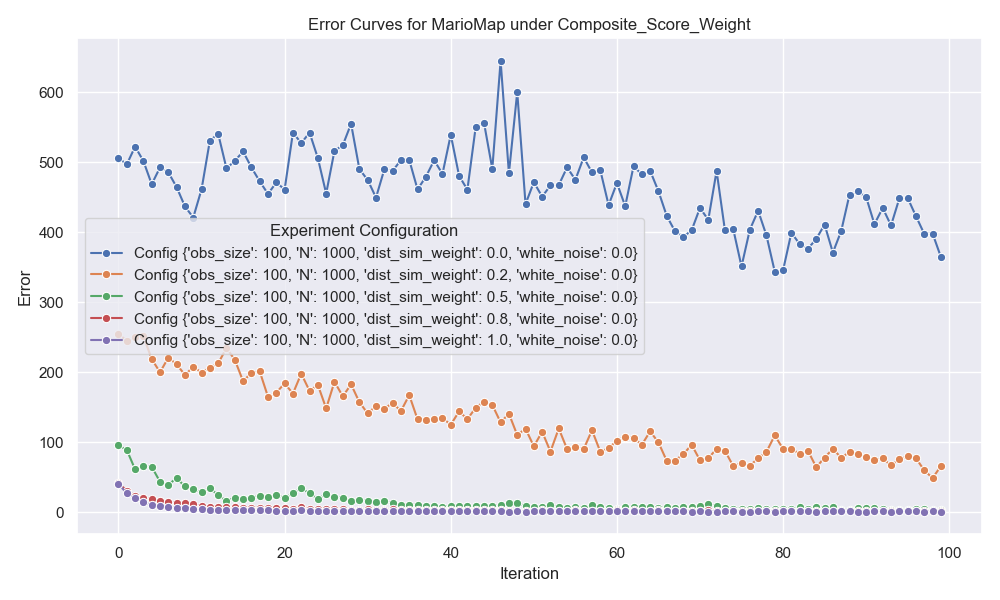
\includegraphics[width=0.49\linewidth]{plots/MarioMap_Composite_Score_Weight.png}\label{fig:mario_scoreweight}}\hspace{0.2cm}%
    \subfigure[Mario Map MSE Curves for Different White Noise Levels] {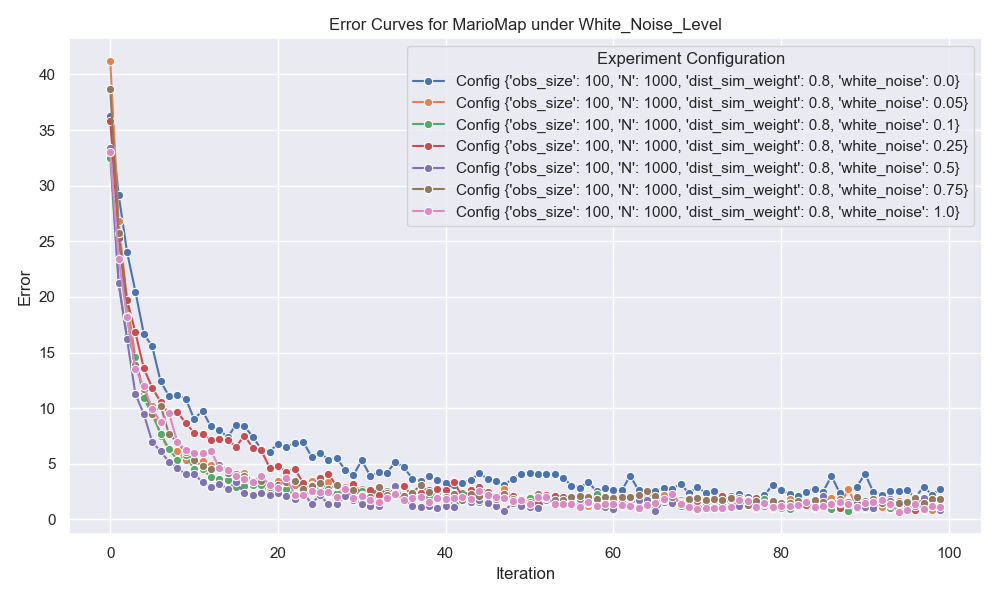
\includegraphics[width=0.49\linewidth]{plots/MarioMap_White_Noise_Level.png}\label{fig:mario_noise}}\hspace{0.2cm}%
    \vspace{-0.4cm}
    \caption{MSE Curves for Mario Map}
    \label{fig:mario}
    \vspace{-0.3cm}
\end{figure*}
As we can see from the results from running the experiments on the Bay map, the variable that influenced the error curve the most is the weight $\gamma$ involved in calculating the composite similarity score between the particles and the GPS location. As can be seen in \ref{fig:bay_scoreweight}, when $\gamma$ is 0.0, the particles never converge to the true location. This is because when $\gamma$ is 0.0, the similarity score becomes equal to the Structural Similarity Index (SSIM) of the particle's image and the reference image. In other words, when $\gamma$ is 0.0, we don't consider the particle's closeness to the GPS location when assiging similarity scores anymore. This makes it hard to filter out particles far away from the true location as SSIM alone is not enough to distinguish a close particle from a far one. Many images far away from the true location can have high SSIM. For the Bay map, the particles tend to end up clustering on top of the ocean regardless of where the true location is when $\gamma$ is 0.0 as shown in \ref{fig:bay_scoreweight0_particles_sample_iter90}.
The next variable that affects the error curve the most is the number of particles. When the number of particles is the lowest (=100), the errors are generally higher than when there are more particles. There are also more spikes in errors when the number of partilces is small. This is not surprising as particles are initialized uniformly randomly and it is less likely that particles happen to be near the true location when there are fewer of them. Observation image sizes and white noise levels don't seem to affect the error curves too much. This adverse effect of reducing the number of partilces is more pronounced on the Mario map as the Mario map is larger than the Bay map so particles are even more sparse. Generally, the variables' effects on the error curves are consistent across maps.
\begin{figure*}[!ht]
    \centering
    \vspace{-0.3cm}
    \subfigure[City Map MSE Curves for Different Observation Image Sizes] {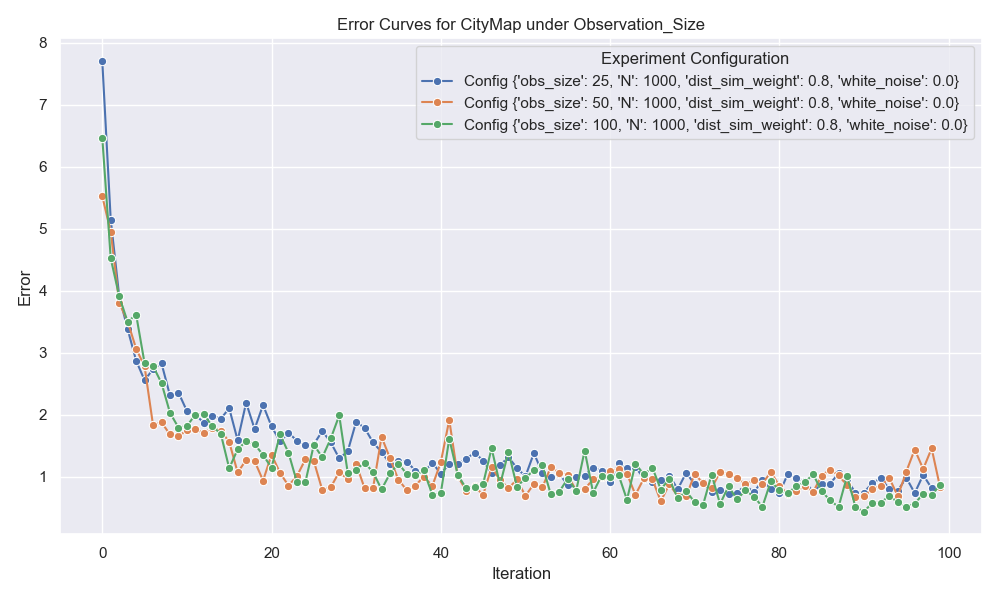
\includegraphics[width=0.48\linewidth]{plots/CityMap_Observation_Size.png}\label{fig:city_obs_size}}\hspace{0.2cm}%
    \subfigure[City Map MSE Curves for Different Particle Number] {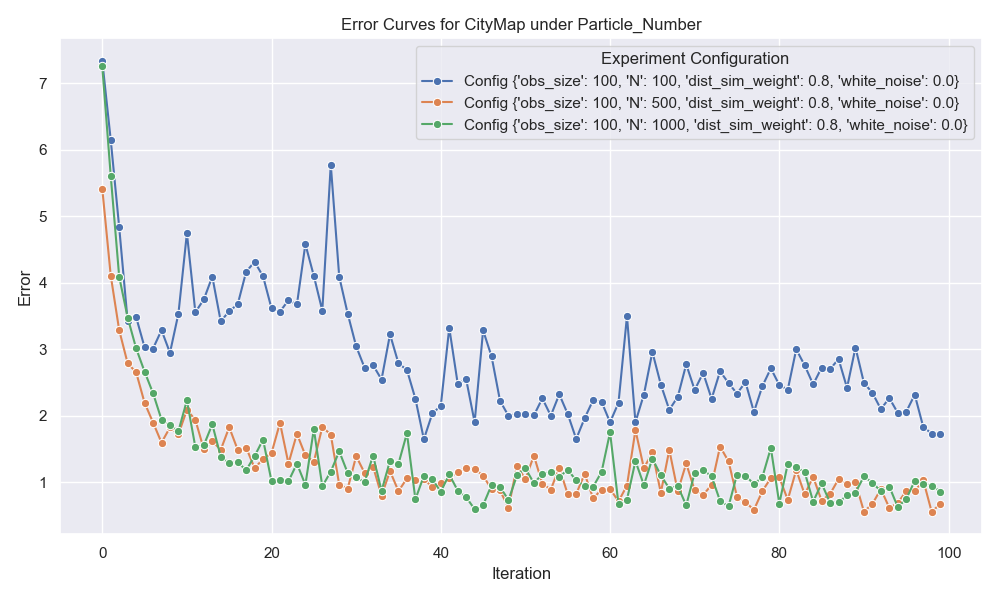
\includegraphics[width=0.49\linewidth]{plots/CityMap_Particle_Number.png}\label{fig:city_pnum}}\hspace{0.2cm}%
    \subfigure[City Map MSE Curves for Different Composite Score Weights] {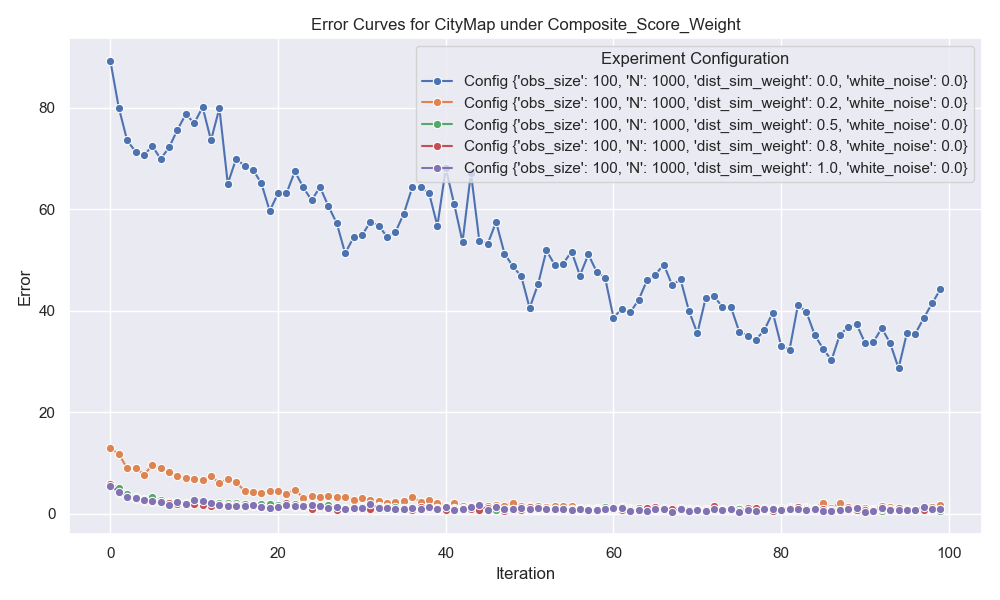
\includegraphics[width=0.49\linewidth]{plots/CityMap_Composite_Score_Weight.png}\label{fig:city_scoreweight}}\hspace{0.2cm}%
    \subfigure[City Map MSE Curves for Different White Noise Levels] {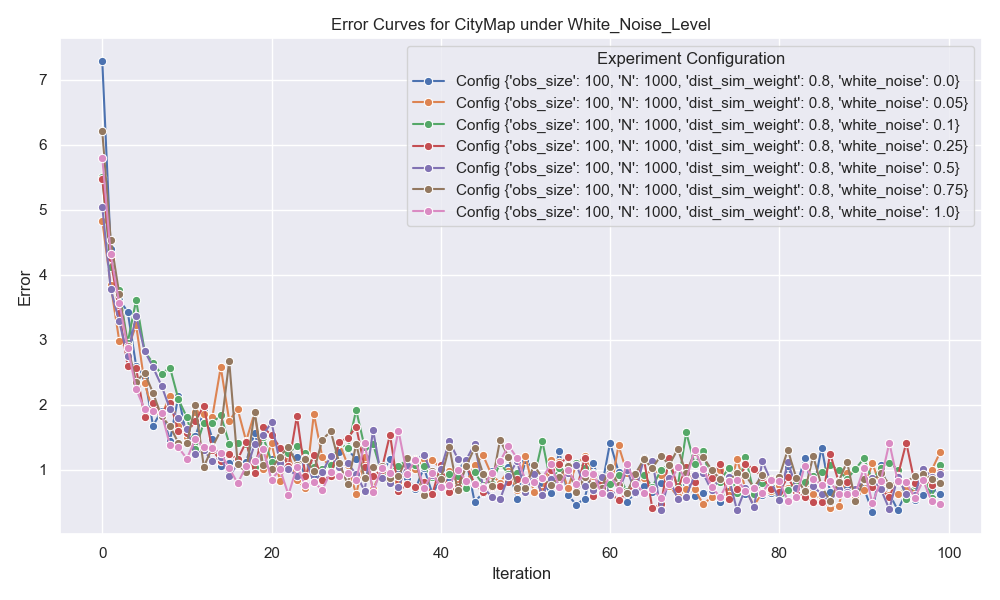
\includegraphics[width=0.49\linewidth]{plots/CityMap_White_Noise_Level.png}\label{fig:city_noise}}\hspace{0.2cm}%
    \vspace{-0.4cm}
    \caption{MSE Curves for City Map}
    \label{fig:city}
    \vspace{-0.3cm}
\end{figure*}
As shown in \ref{fig:mario_scoreweight}, the SSIM measure seems to especially struggle on the Mario map. Not only are the errors generally higher for lower $\gamma$ values, but the particles also fail to cluster around the true locations for $\gamma=0.0$ and $\gamma=0.2$. SSIM is is based on a comparison of three key features: luminance, contrast, and structure. The Mario map is challenging because many observations have similar levels of luminance and contrast, therefore making it hard to distinguish which observation is closer to the reference image. In fact, the ocean in Mario map looks exactly the same everywhere whereas the ocean in Bay map has variations in both luminance and contrast.

White noise not affecting the error curves is not surprising. As the experiment with the composite score weight $\gamma$ demonstrates, the distance-based similarity is the most helpful measure for distinguishing close particles from faraway ones. Since the composite measure is mainly relying on distance to assign particle weights, adding white noise to the reference image should not affect the error curves.  


\begin{figure*}[!ht]
    \centering
    \vspace{-0.2cm}
    \subfigure[Bay Map Particles Initialized at Interation 1] {\includegraphics[width=0.49\linewidth]{BayMap/obs_size100/pnum1000/score_weight0.8/noise0.0/step0resampled.png}\label{fig:bay_obs_size100_particles_sample_iter1.png}}\hspace{0.2cm}%
    \subfigure[Bay Map Particles Iteration 1 With Weights Updated]{\includegraphics[width=0.49\linewidth]{BayMap/obs_size100/pnum1000/score_weight0.8/noise0.0/step0weights.png}\label{fig:bay_obs_size100_particles_weights_iter1.png}}\hspace{0.2cm}%
    \subfigure[Bay Map Particles Iteration 10 With Weights Updated]{\includegraphics[width=0.49\linewidth]{BayMap/obs_size100/pnum1000/score_weight0.8/noise0.0/step10weights.png}\label{fig:bay_obs_size100_particles_weights_iter10.png}}\hspace{0.2cm}%
    \subfigure[Bay Map Particles Iteration 20 With Weights Updated]{\includegraphics[width=0.49\linewidth]{BayMap/obs_size100/pnum1000/score_weight0.8/noise0.0/step20weights.png}\label{fig:fig:bay_obs_size100_particles_weights_iter20.png}}\hspace{0.2cm}%
    \subfigure[Bay Map Particles Iteration 50 With Weights Updated]{\includegraphics[width=0.49\linewidth]{BayMap/obs_size100/pnum1000/score_weight0.8/noise0.0/step50weights.png}\label{fig:fig:bay_obs_size100_particles_weights_iter50.png}}\hspace{0.2cm}%
    \subfigure[Bay Map Particles Iteration 90 With Weights Updated]{\includegraphics[width=0.49\linewidth]{BayMap/obs_size100/pnum1000/score_weight0.8/noise0.0/step90weights.png}\label{ig:fig:bay_obs_size100_particles_weights_iter90.png}}\hspace{0.2cm}%
    \vspace{-0.4cm}
    \caption{Bay Map Particle Filtering}
    \label{fig:bay_particles}
    \vspace{-0.3cm}
\end{figure*}

\begin{figure*}[!ht]
    \centering
    \vspace{-0.4cm}
    \subfigure[Mario Map Particles Initialized at Interation 1] {\includegraphics[width=0.4\linewidth]{MarioMap/obs_size100/pnum1000/score_weight0.8/noise0.0/step0resampled.png}\label{fig:mario_obs_size100_particles_sample_iter1.png}}\hspace{0.2cm}%
    \subfigure[Mario Map Particles Iteration 1 With Weights Updated]{\includegraphics[width=0.4\linewidth]{MarioMap/obs_size100/pnum1000/score_weight0.8/noise0.0/step0weights.png}\label{fig:mario_obs_size100_particles_weights_iter1.png}}\hspace{0.2cm}%
    \subfigure[Mario Map Particles Iteration 10 With Weights Updated]{\includegraphics[width=0.4\linewidth]{MarioMap/obs_size100/pnum1000/score_weight0.8/noise0.0/step10weights.png}\label{fig:mario_obs_size100_particles_weights_iter10.png}}\hspace{0.2cm}%
    \subfigure[Mario Map Particles Iteration 20 With Weights Updated]{\includegraphics[width=0.4\linewidth]{MarioMap/obs_size100/pnum1000/score_weight0.8/noise0.0/step20weights.png}\label{fig:mario_obs_size100_particles_weights_iter20.png}}\hspace{0.2cm}%
    \subfigure[Mario Map Particles Iteration 50 With Weights Updated]{\includegraphics[width=0.4\linewidth]{MarioMap/obs_size100/pnum1000/score_weight0.8/noise0.0/step50weights.png}\label{fig:mario_obs_size100_particles_weights_iter50.png}}\hspace{0.2cm}%
    \subfigure[Mario Map Particles Iteration 90 With Weights Updated]{\includegraphics[width=0.4\linewidth]{MarioMap/obs_size100/pnum1000/score_weight0.8/noise0.0/step90weights.png}\label{fig:mario_obs_size100_particles_weights_iter90.png}}\hspace{0.2cm}%
    \vspace{-0.4cm}
    \caption{Mario Map Particle Filtering}
    \label{fig:mario_particles}
    \vspace{-0.3cm}
\end{figure*}
\begin{figure*}[!ht]
    \centering
    \vspace{-0.3cm}
    \subfigure[City Map Particles Initialized at Interation 1] {\includegraphics[width=\linewidth]{CityMap/obs_size100/pnum1000/score_weight0.8/noise0.0/step0resampled.png}\label{fig:city_obs_size100_particles_sample_iter1.png}}\hspace{0.2cm}%
    \subfigure[City Map Particles Iteration 1 With Weights Updated]{\includegraphics[width=\linewidth]{CityMap/obs_size100/pnum1000/score_weight0.8/noise0.0/step0weights.png}\label{fig:city_obs_size100_particles_weights_iter1.png}}\hspace{0.2cm}%
    \subfigure[City Map Particles Iteration 10 With Weights Updated]{\includegraphics[width=\linewidth]{CityMap/obs_size100/pnum1000/score_weight0.8/noise0.0/step10weights.png}\label{fig:city_obs_size100_particles_weights_iter10.png}}\hspace{0.2cm}%
    \vspace{-0.4cm}
    \caption{City Map Particle Filtering Iteration 1 - 10}
    \label{fig:city_particles_p1}
    \vspace{-0.3cm}
\end{figure*}·
\begin{figure*}[!ht]
    \centering
    \vspace{-0.3cm}
    \subfigure[City Map Particles Iteration 20 With Weights Updated]{\includegraphics[width=\linewidth]{CityMap/obs_size100/pnum1000/score_weight0.8/noise0.0/step20weights.png}\label{fig:city_obs_size100_particles_weights_iter20.png}}\hspace{0.2cm}%
    \subfigure[City Map Particles Iteration 50 With Weights Updated]{\includegraphics[width=\linewidth]{CityMap/obs_size100/pnum1000/score_weight0.8/noise0.0/step50weights.png}\label{fig:city_obs_size100_particles_weights_iter50.png}}\hspace{0.2cm}%
    \subfigure[City Map Particles Iteration 90 With Weights Updated]{\includegraphics[width=\linewidth]{CityMap/obs_size100/pnum1000/score_weight0.8/noise0.0/step90weights.png}\label{fig:city_obs_size100_particles_weights_iter90.png}}\hspace{0.2cm}%
    \vspace{-0.4cm}
    \caption{City Map Particle Filtering Iteration 20 - 90}
    \label{fig:city_particles_p2}
    \vspace{-0.3cm}
\end{figure*}·
\end{document}
